\section{Linguaggi utilizzati}

Si è deciso di utilizzare il modello MVC (Model View Controller) per semplificare la gestione
e diminuire la ridondanza del codice.

\subsection{HTML5}
Il linguaggio di markup \textit{HTML5} è stato utilizzato per la parte View del modello.

Per ridurre la ridondanza, la struttura html e' stata "smontata" in diversi file (Header, Breadcrimb, Main, Footer ecc..),
questi file hanno solo una struttura base e non contengono alcuna informazione.  Una pagina viene 
riscostrutita utilizzando il codice \textit{PHP}, il quale prende i file html, inserisce dentro le informazioni della pagina da
visualizzare e ricompone i file per formare una pagina completa.

\subsection{PHP}
Il lato server, che corrisponde anche alla parte controller, è stato sviluppato utilizzando il linguaggio di programmazione \textit{PHP}.

Esso ricopre un ruolo fondamentale. Come detto sopra, deve ricostruire una pagina completa 
inserendo nei file le informazioni; infatti ogni pagina del sito ha un file \textit{"index.php"} che funge 
da costruttore della pagina e in base al funzionamento, ci sono ulteriori file che gestiscono le azioni fatte
dagli utenti.


\subsection{CSS}
E' stato utilizzato il linguaggio di formattazione \textit{CSS} per modellare il layout sito.

Sono stati prodotti 3 fogli di stile:
\begin{itemize}
	\item \textit{index.css}: foglio di stile principale;
	\item \textit{mini.css}: foglio di stile per schermi di piccole dimensioni;
	\item \textit{print.css}: foglio di stile per la stampa.
\end{itemize}

\subsection{SQL}
\textit{SQL} è stato utilizzato nella crazione del database, il quale è formato dalle seguenti tabelle:

\begin{itemize}
	\item \textit{Brand}: si riferisce alla marca del dispositivo;
	\item \textit{Model}: contiene le informazioni del modello di una marca;
	\item \textit{Purchase item}: contiene informazioni relative agli acquisti, dispositivi venduti e non;
	\item \textit{Repair item}: contiene informazioni relative alle riparazioni, comprese le riparazioni effettuate e non;
	\item \textit{User}: contiene informazioni degli utenti;
\end{itemize}

Le tabelle \textit{Brand} e \textit{Model} sono già riempite con dataset; invece le tabelle \textit{Purchase item} e \textit{Repair item}
verranno riempite man mano che gli utenti eseguono le richieste.

\begin{figure}[H]
	\centering
	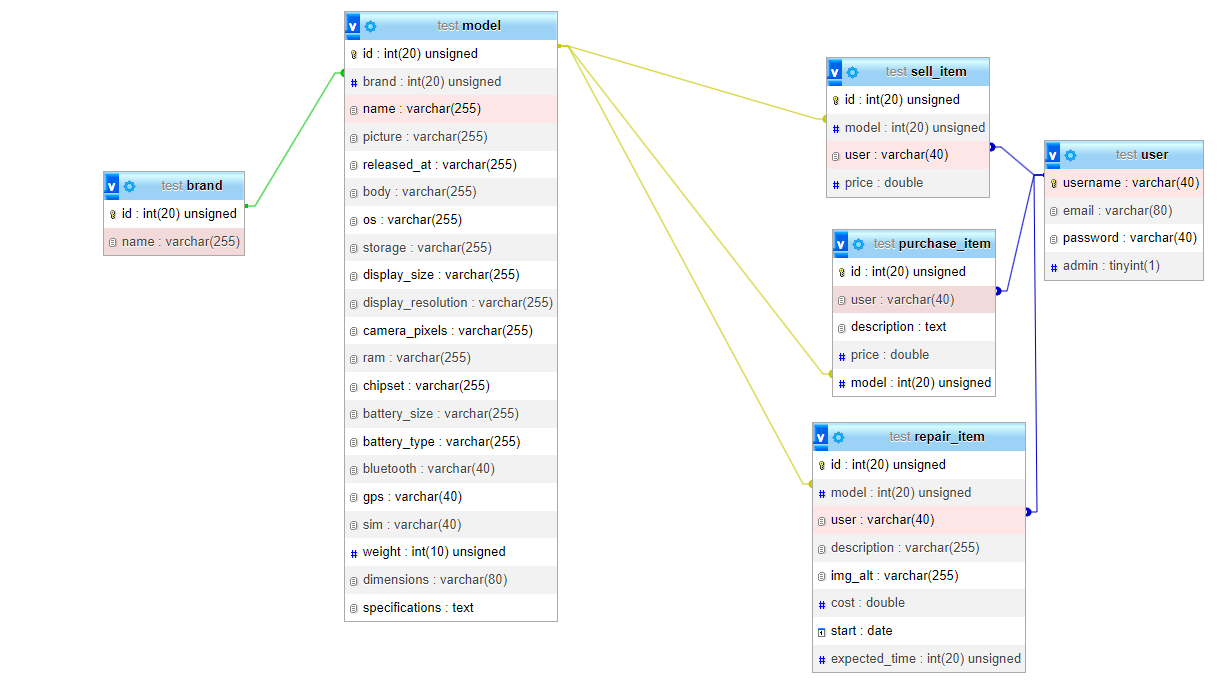
\includegraphics[scale=0.4]{res/database.png}
	\caption{Modello del database}
\end{figure}

\subsection{JavaScript}
\textit{JavaScript} è stato utilizzato per rendere il sito piu' dinamico e migliorare l’esperienza utente. Occorre
precisare però che la sua disabilitazione o il suo mancato funzionamento non comportano in alcun
modo l’impossibilit`a di fruire dei servizi offerti dal sito.

Innazitutto viene utilizzato per applicazione di una rappresentazione di una serie di immagini, visualizzandole
una alla volta attraverso due pulsanti \textit{precedente} e \textit{successivo}; si può trovare un esempio d'uso
nella pagina principale.

Un suo secondo utilizzo è rendere visibile un pulsante a freccia in su che ha il compito di riportare l'utente
in cima alla pagina. Il punsante ovviamente diventa visibile e cliccabile quando l'utente ha scrollato(SI PUO DIRE?) la pagina in giu'

Infine viene utilizzato per controllare gli input tipo per Login e Registrazione, dove neccessitano di un controllo del formato
del testo inserito; in caso del formato sbagliato verrà visualizzata un suggerimento sotto al box di inserimento sul formato del
testo accettato